\documentclass[a4paper]{article}
\usepackage[a4paper,margin=0mm]{geometry}
\usepackage{fontspec}
\usepackage{unicode-math}
\usepackage{tikz}
\usetikzlibrary{fit,calc,positioning}
\usepackage[table]{xcolor}
\usepackage[absolute]{textpos}
\usepackage{array}

\setmainfont{Libertinus Serif}
\setsansfont{Libertinus Sans}
\setmathfont{Libertinus Math}

\definecolor{accent}{HTML}{F46530}
\definecolor{badge}{HTML}{FFBDA5}
\definecolor{ink}{HTML}{2A2E30}

\setlength{\TPHorizModule}{1mm}
\setlength{\TPVertModule}{1mm}
\setlength{\parindent}{0pt}
\pagestyle{empty}

\newcommand{\topicheader}[2]{%
\begin{textblock*}{194mm}(16mm,10mm)
\begin{tikzpicture}
\node[fill=accent,text=white,font=\sffamily\bfseries\fontsize{13}{13}\selectfont,
      minimum width=9mm,minimum height=9mm,inner sep=0pt] at (4.5mm,-4.5mm) {#1};
\node[font=\sffamily\bfseries\fontsize{15}{16}\selectfont,text=ink,anchor=west] at (12mm,-4.5mm) {#2};
\end{tikzpicture}
\end{textblock*}
\begin{textblock*}{194mm}(16mm,22.5mm)

\begin{tikzpicture}
\fill[accent] (0,0) rectangle (194mm,0.5mm);
\end{tikzpicture}
\end{textblock*}
}

\newcommand{\pagekicker}[1]{%
\begin{textblock*}{100mm}(16mm,25.5mm)
\begin{tikzpicture}
\node[fill=ink,text=white,font=\sffamily\bfseries\fontsize{8}{8}\selectfont,
      inner sep=2.2pt,rounded corners=1pt] {\MakeUppercase{#1}};
\end{tikzpicture}
\end{textblock*}
}

\newcommand{\pagefooter}[1]{%
\begin{textblock*}{194mm}(8mm,286.41mm)
  
\begin{tikzpicture}
    \fill[accent] (0,0) rectangle (194mm,0.6mm);
  \end{tikzpicture}
\end{textblock*}
\begin{textblock*}{63.59mm}(8mm,288.27mm)
  {\sffamily\bfseries\color{accent}\fontsize{13}{16}\selectfont SAT 1200+}
\end{textblock*}
\begin{textblock*}{10mm}(188mm,288.27mm)
  \centering{\sffamily\color{accent}\fontsize{14}{16}\selectfont #1}
\end{textblock*}
}

\newcommand{\cardbg}[4]{%
\begin{textblock*}{#3mm}(#1mm,#2mm)
\begin{tikzpicture}
\fill[badge!22,rounded corners=3mm] (0,0) rectangle (#3mm,-#4mm);
\end{tikzpicture}
\end{textblock*}%
}

\newcommand{\pill}[3]{%
\begin{textblock*}{160mm}(#1mm,#2mm)
\begin{tikzpicture}
\node[fill=accent,text=white,anchor=north west,font=\sffamily\bfseries\fontsize{10}{10}\selectfont,
      rounded corners=8pt,inner xsep=5mm,inner ysep=1.8mm] at (0,0) {QOIDA ~\textperiodcentered~ #3};
\end{tikzpicture}
\end{textblock*}%
}

\arrayrulecolor{accent}
\setlength{\arrayrulewidth}{0.7pt}
\renewcommand{\arraystretch}{1.5}

\begin{document}

\topicheader{6}{Bir noma'lumli tenglamalar}
\pagekicker{Formula sheet}
\pagefooter{32}
\mbox{}%

% ================= CARD A: Bir qadamli (left) / Ikki qadamli (right) (y: 33-91) =================
\cardbg{16}{33}{85}{58}
\pill{22}{36}{Bir qadamli}

\begin{textblock*}{75mm}(20mm,52mm)
\begin{center}
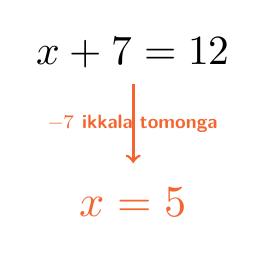
\begin{tikzpicture}
\node[font=\fontsize{15}{15}\selectfont] (eq) at (0,0) {$x+7=12$};
\node[font=\sffamily\bfseries\scriptsize,text=accent] at (0,-9mm) {$-7$ ikkala tomonga};
\node[font=\fontsize{16}{16}\selectfont,text=accent] at (0,-19mm) {$x=5$};
\draw[accent,->,line width=1pt] (0,-4mm) -- (0,-14mm);
\end{tikzpicture}
\end{center}
\end{textblock*}

\cardbg{109}{33}{85}{58}
\pill{115}{36}{Ikki qadamli}

\begin{textblock*}{75mm}(113mm,49mm)
\begin{center}
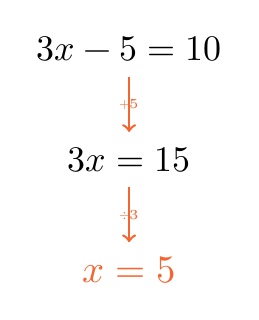
\begin{tikzpicture}
\node[font=\fontsize{13}{13}\selectfont] (e0) at (0,0) {$3x-5=10$};
\node[font=\sffamily\bfseries\tiny,text=accent] at (0,-7mm) {$+5$};
\node[font=\fontsize{13}{13}\selectfont] (e1) at (0,-14mm) {$3x=15$};
\node[font=\sffamily\bfseries\tiny,text=accent] at (0,-21mm) {$\div3$};
\node[font=\fontsize{14}{14}\selectfont,text=accent] (e2) at (0,-28mm) {$x=5$};
\draw[accent,->,line width=0.9pt] (0,-3.5mm) -- (0,-10.5mm);
\draw[accent,->,line width=0.9pt] (0,-17.5mm) -- (0,-24.5mm);
\end{tikzpicture}
\end{center}
\end{textblock*}

% ================= CARD B: Ko'p qadamli -- qavs ochish (y: 97-185) =================
\cardbg{16}{97}{178}{88}
\pill{26}{100}{Ko'p qadamli: qavs ochish}

\begin{textblock*}{158mm}(26mm,111mm)
{\fontsize{11}{14}\selectfont\color{ink}
Avval qavsni oching va o'xshash hadlarni ixchamlashtiring -- shundan keyin oddiy ikki qadamli tenglama qoladi:}
\end{textblock*}

\begin{textblock*}{158mm}(26mm,124mm)
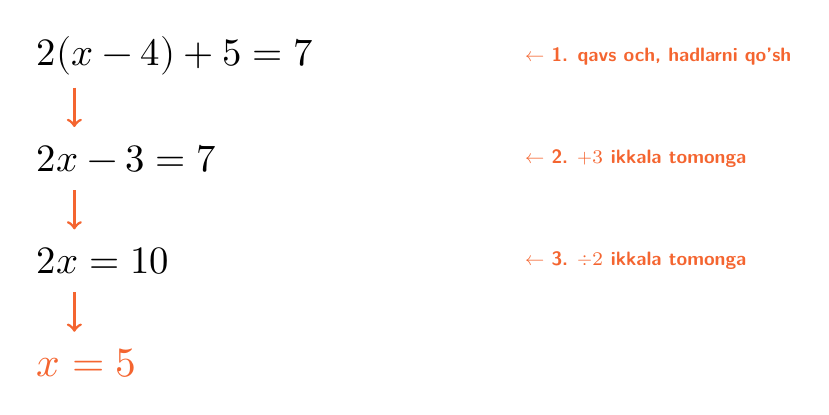
\begin{tikzpicture}[every node/.style={font=\fontsize{14}{14}\selectfont}]
\node[anchor=west] (l0) at (0,0) {$2(x-4)+5=7$};
\node[anchor=west,font=\sffamily\bfseries\scriptsize,text=accent] at (62mm,0) {$\leftarrow$ 1. qavs och, hadlarni qo'sh};

\node[anchor=west] (l1) at (0,-13mm) {$2x-3=7$};
\node[anchor=west,font=\sffamily\bfseries\scriptsize,text=accent] at (62mm,-13mm) {$\leftarrow$ 2. $+3$ ikkala tomonga};

\node[anchor=west] (l2) at (0,-26mm) {$2x=10$};
\node[anchor=west,font=\sffamily\bfseries\scriptsize,text=accent] at (62mm,-26mm) {$\leftarrow$ 3. $\div2$ ikkala tomonga};

\node[anchor=west,font=\sffamily\bfseries\fontsize{15}{15}\selectfont,text=accent] (l3) at (0,-39mm) {$x=5$};

\foreach \y in {-4,-17,-30}{
  \draw[accent,->,line width=1pt] (6mm,\y mm) -- (6mm,\y mm -5mm);
}
\end{tikzpicture}
\end{textblock*}

% ================= CARD C: Ikkala tomonda noma'lum (y: 191-279) =================
\cardbg{16}{191}{178}{88}
\pill{26}{194}{Ikkala tomonda noma'lum}

\begin{textblock*}{158mm}(26mm,205mm)
{\fontsize{11}{14}\selectfont\color{ink}
Noma'lumli hadlarni bir tomonga, sonli hadlarni ikkinchi tomonga yig'ing:}
\end{textblock*}

\begin{textblock*}{158mm}(26mm,218mm)
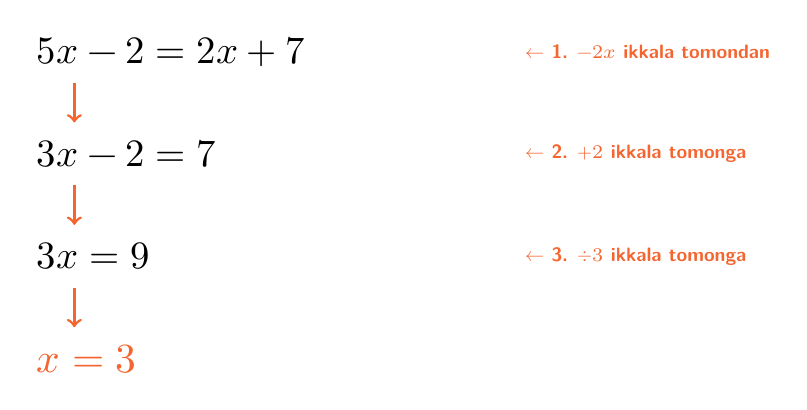
\begin{tikzpicture}[every node/.style={font=\fontsize{14}{14}\selectfont}]
\node[anchor=west] (m0) at (0,0) {$5x-2=2x+7$};
\node[anchor=west,font=\sffamily\bfseries\scriptsize,text=accent] at (62mm,0) {$\leftarrow$ 1. $-2x$ ikkala tomondan};

\node[anchor=west] (m1) at (0,-13mm) {$3x-2=7$};
\node[anchor=west,font=\sffamily\bfseries\scriptsize,text=accent] at (62mm,-13mm) {$\leftarrow$ 2. $+2$ ikkala tomonga};

\node[anchor=west] (m2) at (0,-26mm) {$3x=9$};
\node[anchor=west,font=\sffamily\bfseries\scriptsize,text=accent] at (62mm,-26mm) {$\leftarrow$ 3. $\div3$ ikkala tomonga};

\node[anchor=west,font=\sffamily\bfseries\fontsize{15}{15}\selectfont,text=accent] (m3) at (0,-39mm) {$x=3$};

\foreach \y in {-4,-17,-30}{
  \draw[accent,->,line width=1pt] (6mm,\y mm) -- (6mm,\y mm -5mm);
}
\end{tikzpicture}
\end{textblock*}

\end{document}
